\chapter*{Ubiquitous Language}

Think about a recent project that you worked on. Sometimes a word (or phrase) will only be used by the business. Others may only be used by developers and testers. Some are used by the whole team.
At your table discuss those terms. Write the terms in this Venn diagram:

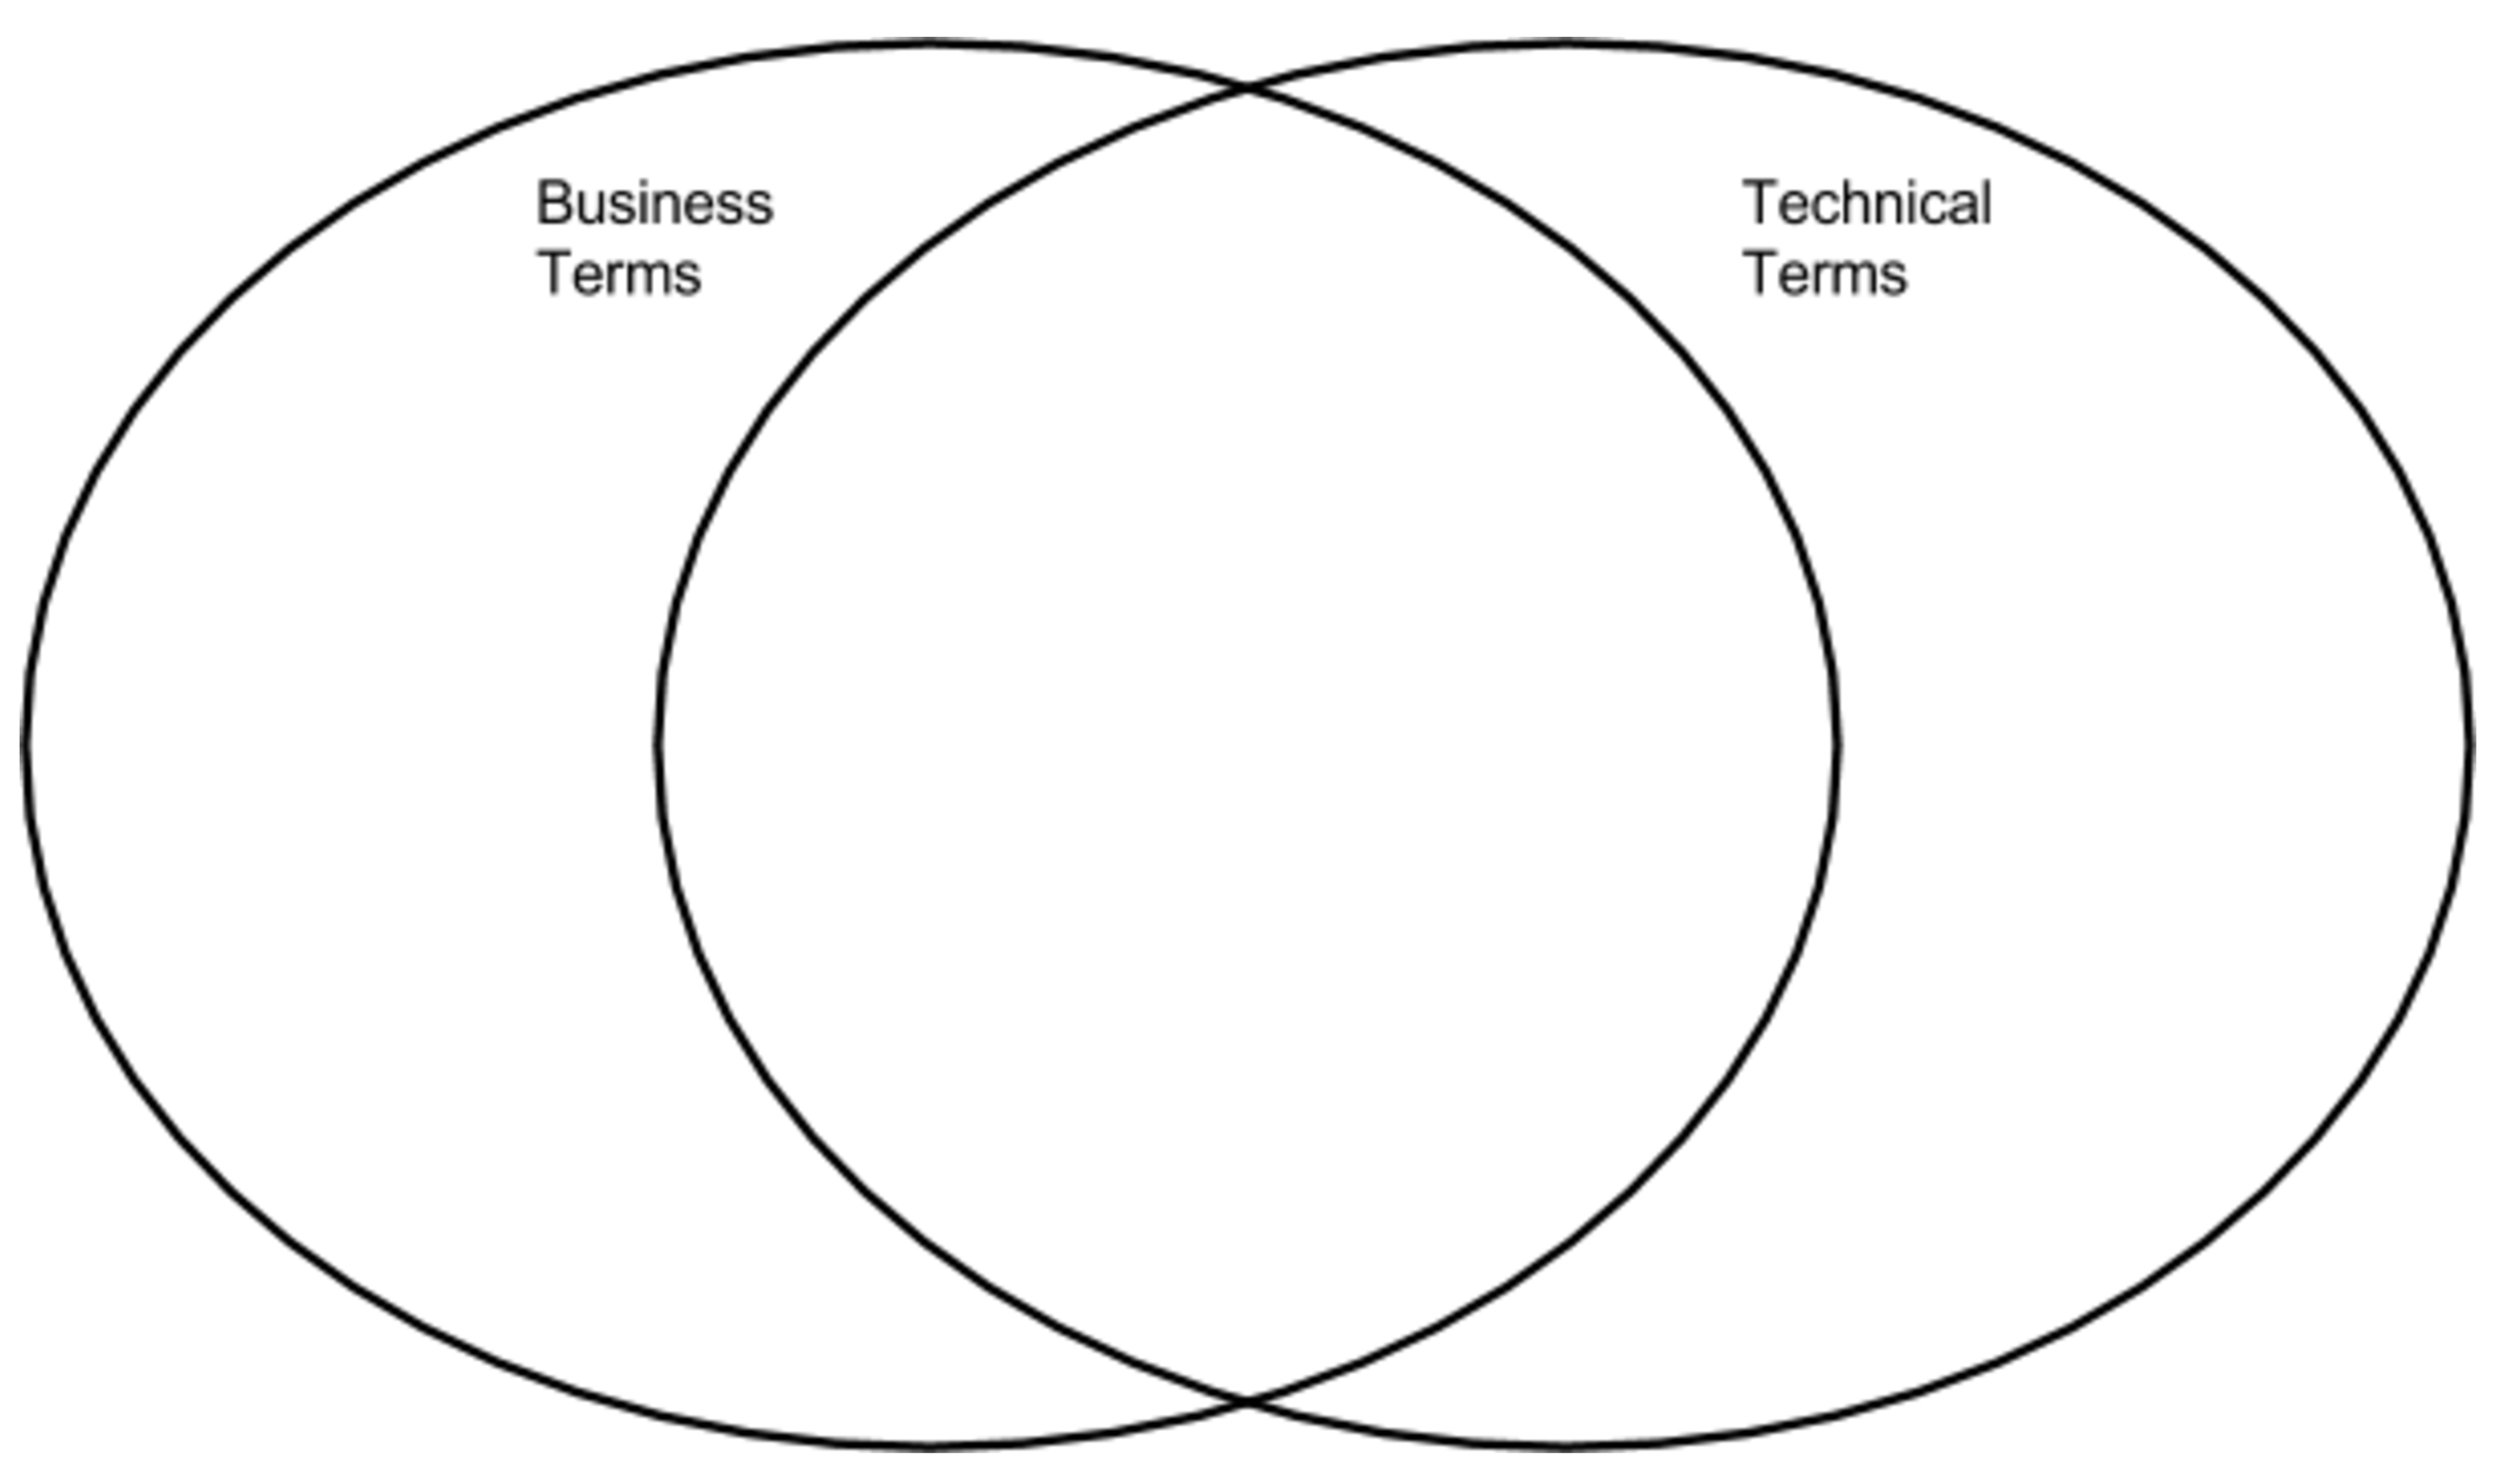
\includegraphics[width=\textwidth]{images/ubiquitous-venn}

Look at the terms that are shared between the business and technical domains. Are any of them imprecise or ambiguous? Could they be interpreted differently by different team members?

\answerbox{1.3}

Did your project team create any new terms, especially to help business and technical people to communicate about something you didn't have a word for?

\answerbox{1.3}

What would be the consequences if everyone on your project team used the same words, right from your specification documents to your database tables?

\answerbox{1.3}
